%================
%   Part A
%================

{\LARGE A:}
Which filter needs the highest order? Which is the lowest?\\

Butterworth N: 11\\
Chebyshev N: 6\\
Elliptic N: 4\\

ButterWorth has the highest order while Elliptic has the Lowest.\\ \\ 


{\LARGE C:}
Can you explain the features of the frequency responses from the poles and zeros?\\

For the ButterWorth Filter all the zeros corespond to real -1 while all the poles circle around real 1 and in the imaginary domain.\\

For the Chebyshev Filter the zeros wrapped around the imaginary 1 and -1 while the poles get closer to 0 in both the real and imaginary point.\\

For the Elliptic Filter the zeros are around the imaginary domain leaning towards the positive real side. The poles around the positive real. 


\begin{homeworkProblem}
\begin{center}
\lstinputlisting{problem9_5.m}{Code 2: matlab script for Problem 5}
\end{center}

\begin{figure}[!htbp]
  \centering
    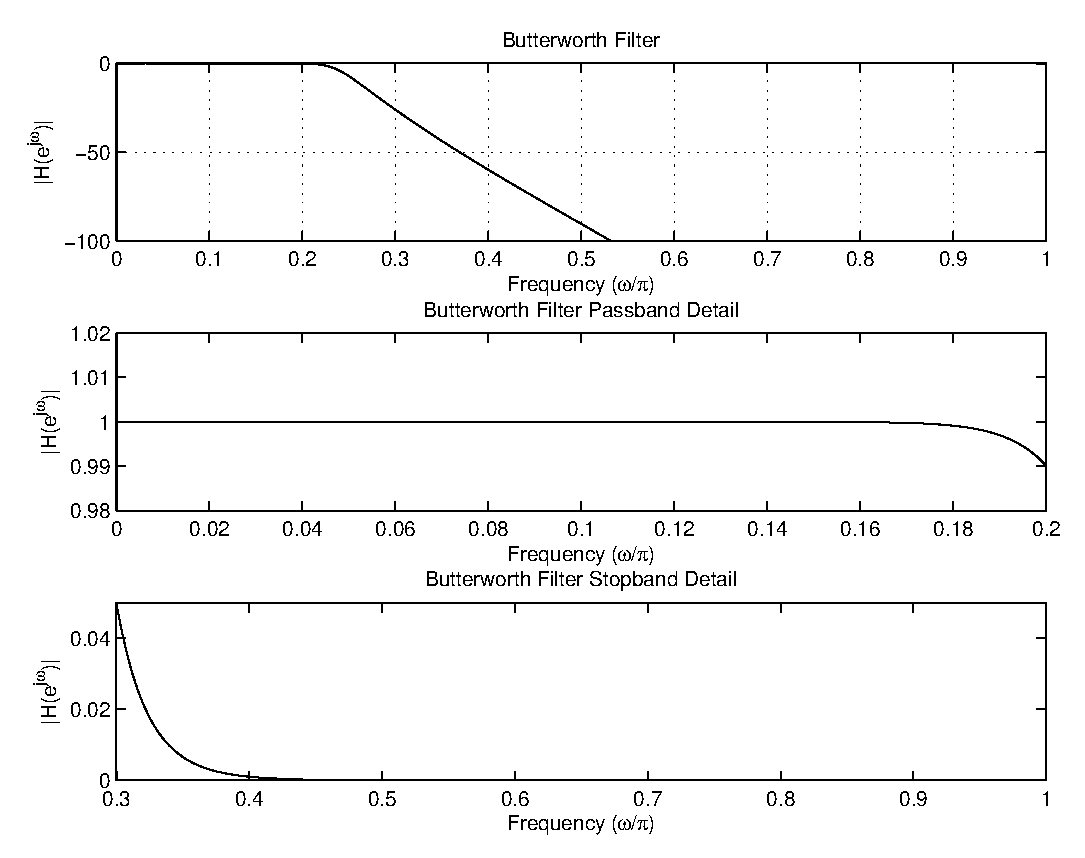
\includegraphics[width=0.7\textwidth]{Figures/PS9-5-1.eps}
  \caption{ButterWorth Filter}
\end{figure}

\begin{figure}[!htbp]
  \centering
    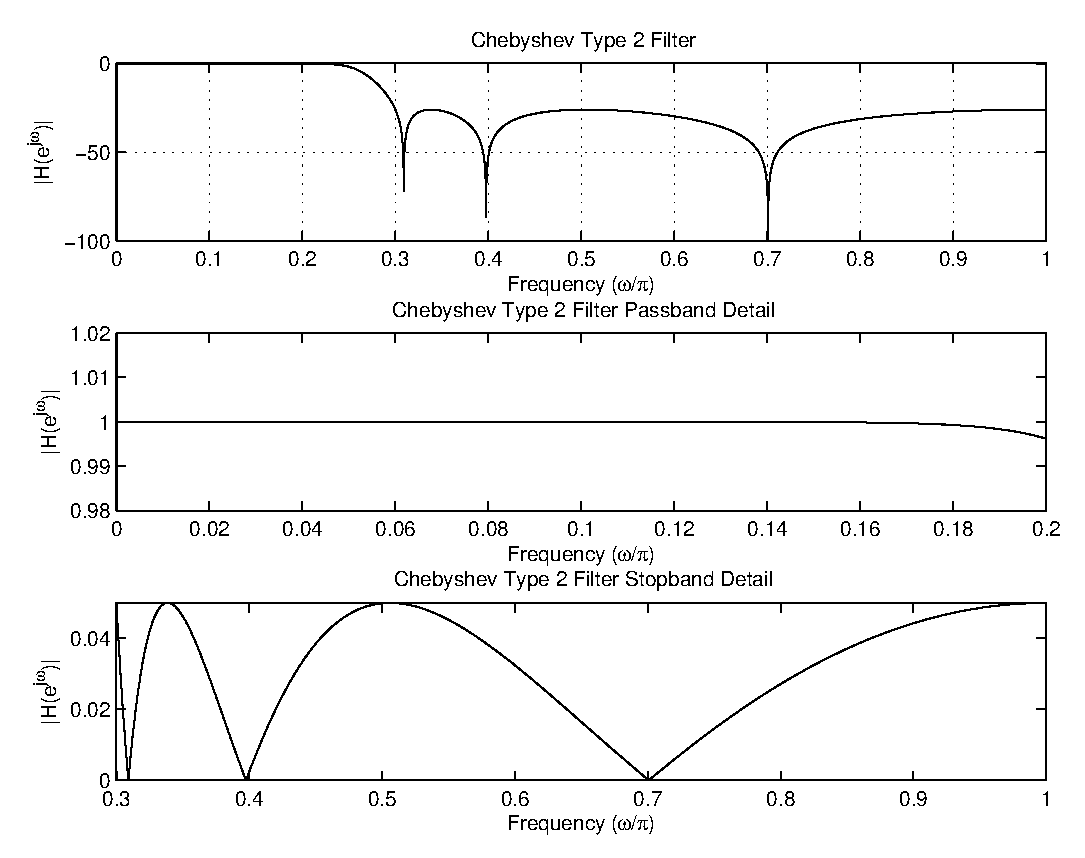
\includegraphics[width=0.7\textwidth]{Figures/PS9-5-2.eps}
  \caption{Chebyshev Filter}
\end{figure}

\begin{figure}[!htbp]
  \centering
    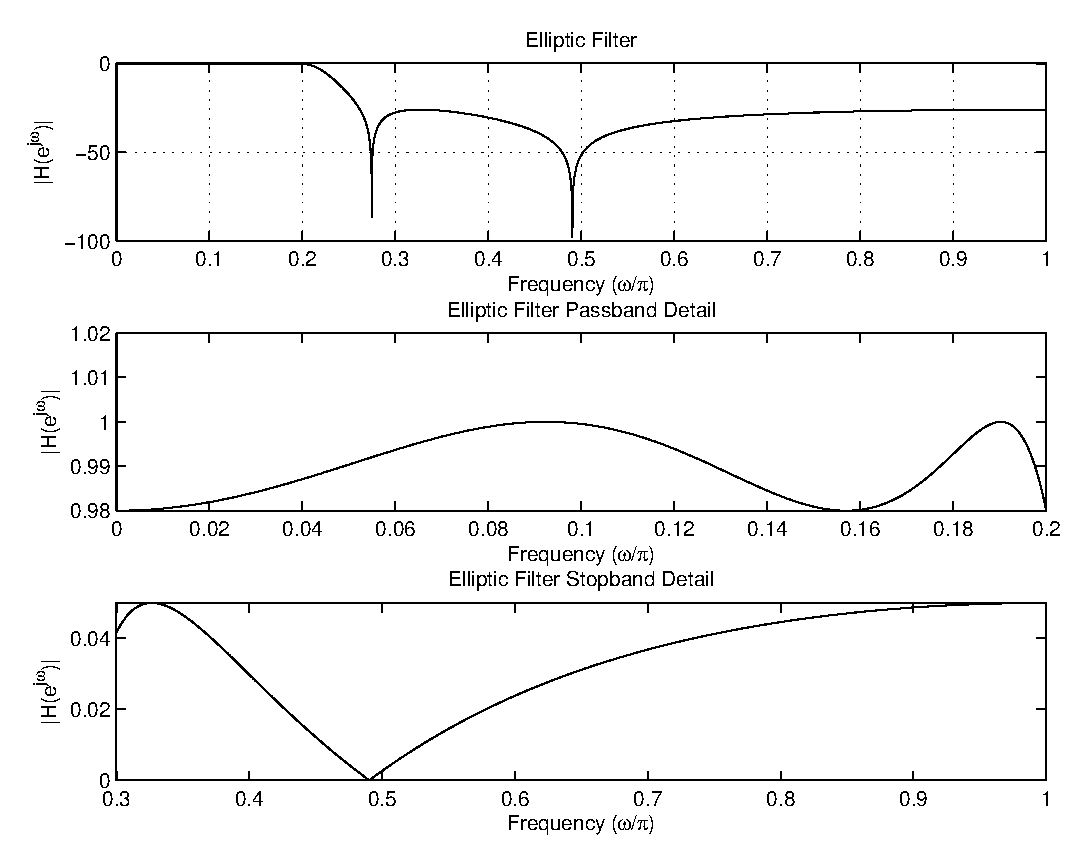
\includegraphics[width=0.7\textwidth]{Figures/PS9-5-3.eps}
  \caption{Elliptic Filter}
\end{figure}

\begin{figure}[!htbp]
  \centering
    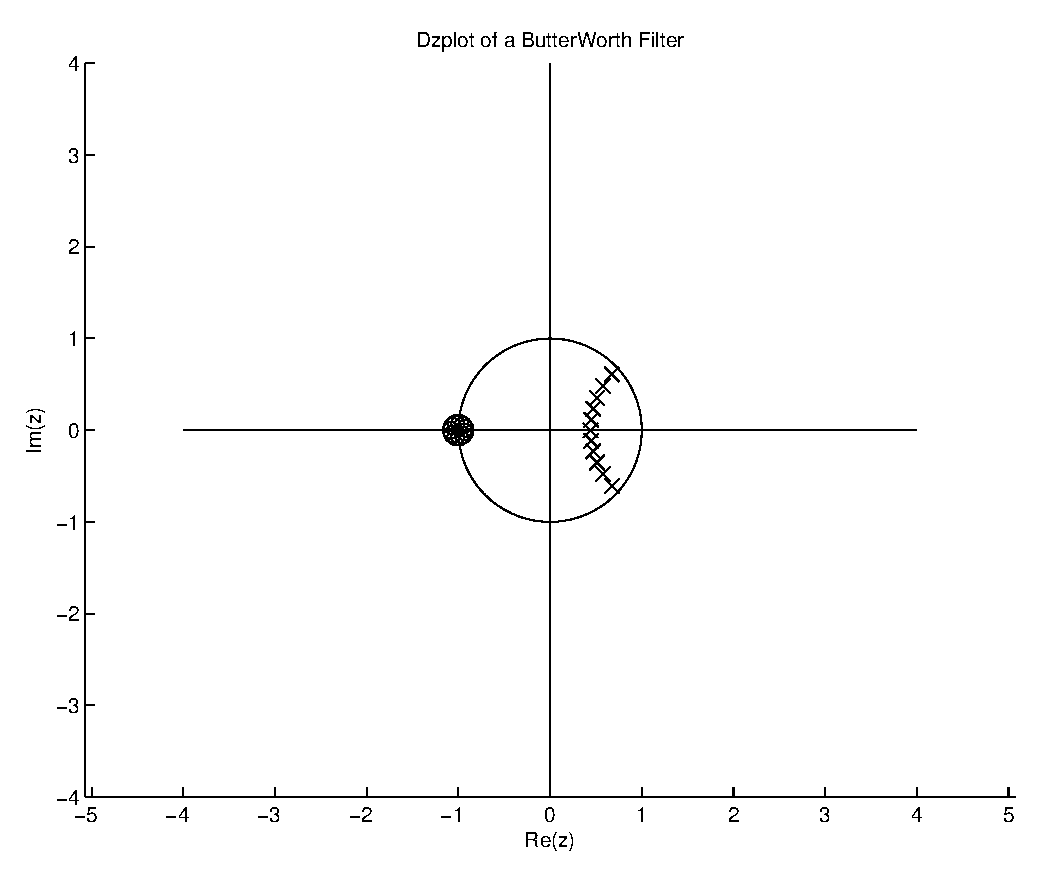
\includegraphics[width=0.7\textwidth]{Figures/PS9-5-4.eps}
  \caption{ButterWorth Zeroplot}
\end{figure}

\begin{figure}[!htbp]
  \centering
    \includegraphics[width=0.7\textwidth]{Figures/PS9-5-5.eps}
  \caption{Chebyshev Zeroplot}
\end{figure}

\begin{figure}[!htbp]
  \centering
    \includegraphics[width=0.7\textwidth]{Figures/PS9-5-6.eps}
  \caption{Elliptic Zeroplot}
\end{figure}



\end{homeworkProblem}

